%% Exemple de source LaTeX pour un article soumis à TALN 2018
\documentclass[10pt,twoside]{article}

\usepackage{times}
\usepackage[utf8]{inputenc}
\usepackage[T1]{fontenc}
\usepackage{graphicx}

% faire les \usepackage dont vous avez besoin AVANT le \usepackage{taln2018}

\usepackage{taln2018}
\usepackage[frenchb]{babel}

% Titre complet
\title{Extraction automatique et visualisation de termes de maintenance pour le peuplement d'ontologies métiers}

\author{Meryl Bothua\quad Laurent Pierre\\
  {\small
    EDF Lab Paris-Saclay,7 bd Gaspard Monge, 91120 PALAISEAU, France\\
    \texttt{
      meryl.bothua@edf.fr, laurent.pierre@edf.fr \\
}}}


\begin{document}
\maketitle

\resume{EDF a développé une chaîne logicielle destinée à extraire et analyser l’information contenue dans les rapports de maintenance. Les expériences menées avec Word2Vec nous ont permis de créer des ressources lexicales à partir de ces documents. Grâce à celles-ci, nous peuplons des ontologies et visualisons les résultats à l’aide d’un outil de navigation dans des graphes RDF. Nous avons mis en place un processus semi-automatique de correction et de validation des termes lexicaux destinés à peupler l’ontologie métier finale.
}

\abstract{Automated Extraction and Visualization of Terms Related to Maintenance in Order to Populate Business Ontologies}{
EDF is developing a process dedicated to extract and analyze information from maintenance reports.  Experiments with Word2Vec were conducted for creating lexical resources from these sets of documents.  We populated ontologies from the Word2Vec outputs in order to visualize and check the accuracy of the results, thanks to our ontology driven RDF graph UI.  We describe the semi\-automation of the processing line dedicated to correction and validation of lexical terms intended to populate the final business ontology.
}

\motsClefs
  {similarité entre mots, plongement de mots, visualisation de données, recherche d'informations, peuplement d'ontologie}
  {word similarity, word embedding, data visualization, information retrieval, ontology population}


\section{Introduction}

EDF est aujourd’hui au coeur de la transition numérique et mène de nombreuses études sur l’exploitation de données diverses. Dans cette optique, des méthodes de fouille de texte sont testées afin d’exploiter les données non structurées. Une chaîne de traitement a été mise en place pour extraire et analyser des informations à partir de rapports de maintenance. Des tests ont permis de mettre en évidence l’apport de Word2Vec \cite{DBLP:journals/corr/abs-1301-3781} pour l’aide à la constitution de ressources lexicales. L’automatisation du processus met en exergue des éléments auparavant noyés dans la masse des données. Le gain est double : une économie de temps est réalisée grâce à la proposition de termes candidats au peuplement de lexiques ; nous produisons actuellement une sortie RDF avec une ontologie dédiée et proposons une visualisation sous forme de graphe avec l’outil SemVue. Pour chaque terme du corpus, des candidats sont donnés après prétraitements. Le gain est également qualitatif : des synonymes, des abréviations, des possibles fautes d’orthographe et des phénomènes de multilinguisme sont retournés par le système. Nous développons actuellement une application web, CuriosiText, pour l’aide au peuplement d’ontologie par des utilisateurs non experts.


\section{Contexte de l'étude}
Une chaîne de traitement de fouille de texte a été mise en place en 2017 à l’aide de la plateforme GATE (General Architecture for Text Engineering). Cette chaîne a pour objectif d’extraire automatiquement des actions de maintenance réalisées sur des composants (exemple : remplacement de l’anémomètre). Dans un premier temps et afin de démontrer la faisabilité de notre cas d’étude, les gazetteers (ou dictionnaires) de cette chaîne ont été développés manuellement. Des experts les ont constitués en pointant les termes pertinents d’une partie du corpus des comptes rendus de maintenance. En vue du passage à l’échelle, nous avons cherché à automatiser cette étape coûteuse en temps ; nous avons ainsi adopté la méthode Word2Vec pour extraire automatiquement les termes similaires sur l’ensemble du corpus et augmenter le rappel de la chaîne de traitement.


\section{Extraction de termes avec Word2Vec}

\subsection{Présentation des données}
Nous avons entraîné un modèle Word2Vec sur un corpus de comptes rendus de maintenance. Ce corpus contient environ 8000 fiches de maintenance. Si la taille de ce corpus semble restreinte, nous avons néanmoins obtenu des résultats concluants (fig \ref{fig:w2v}), les textes étant très répétitifs. En effet, la taille de notre dictionnaire est d'environ 5000 mots après prétraitements. Nous avons également calculé l'indice de richesse lexicale \cite{McKee2000}, quotient entre le nombre d’occurrences d’un token et le nombre total de tokens du texte. Un token est défini comme formé exclusivement de caractères alphabétiques, sans distinguer majuscules et minuscules. Notre corpus comprend 97 065 tokens dont 5887 tokens uniques donnant une richesse lexicale de 0.0607 avant prétraitements.


\subsection{Algorithme}

Nous avons mis en place un script python qui effectue plusieurs opérations. Il est ainsi possible de charger un corpus local ou de récupérer des données externes avec Elasticsearch\footnote{www.elastic.co}.
Un ensemble de prétraitements est ensuite appliqué sur les données à savoir la suppression des caractères non désirés, le découpage en phrases et en mots. Concernant ces deux dernières étapes, nous avons utilisé la fonction dédiée du package NLTK. Nous sommes également partis de l'hypothèse que l'apprentissage de Word2Vec serait plus fin avec l'ajout de métadonnées grammaticales sur les mots de notre corpus. Nous avons donc intégré TreeTagger \cite{Schmid94probabilisticpart-of-speech} à nos traitements pour un étiquetage morphosyntaxique : Word2Vec apprend ainsi sur la forme, le lemme et la catégorie grammaticale du terme. Nous considérons qu'il s'agit d'une première étape de désambiguïsation. À la suite de TreeTagger, les mots vides sont supprimés et nous appelons Word2Vec pour le calcul de la similarité. Une sortie contenant les résultats de Word2Vec au format RDF est alors générée. Cette dernière étape permet de créer une base de connaissance sur les résultats du traitement des documents du corpus contenant les phrases et mots qu'elles contiennent et pour chaque mot du corpus : son label, sa fréquence, sa catégorie morphosyntaxique, son lemme, les 15 premières phrases dans lesquelles il apparaît et les 15 candidats termes les plus similaires (fig \ref{gtype}).


\section{Exploration de termes sous forme de graphe RDF}

Afin de visualiser les résultats de Word2Vec formatés en RDF, nous avons créé une première ontologie modélisée sur Word2Vec. Elle est un premier palier en vue du peuplement d'ontologies métiers.

\begin{figure}[tb]
    \begin{center}
        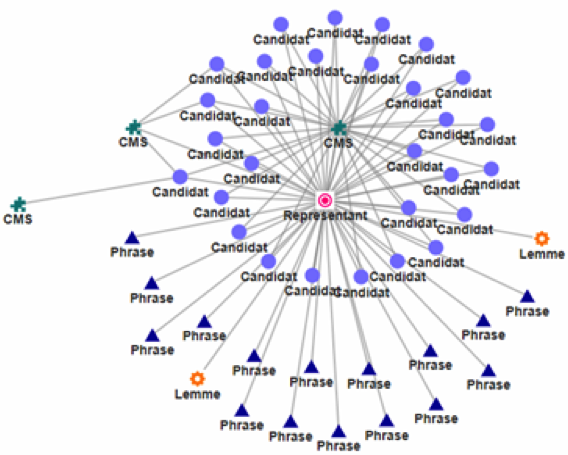
\includegraphics[width=6cm]{figures/gtype}
    \end{center}
    \caption{Graphe Type de l’ontologie pour Word2Vec}\label{fig:gtype}
\end{figure}


Nous souhaitions une visualisation sous forme de graphe où pour chaque mot du corpus, considéré comme étant un Représentant, nous affichons ses quinze Candidats Termes les plus similaires.

Pour visualiser ces résultats, nous avons utilisé l'outil SemVue développé en 2014 à EDF. Cet outil propose une interface de navigation dans un graphe RDF extrêmement facile à mettre en œuvre à chaque étape du développement d’un entrepôt de données. Le cœur de l’interface est défini à l’aide d’une ontologie associée à la modélisation métier proprement dite dans un entrepôt de données \cite{mnpho14parallel-materialisation-RDFox} et permet ainsi à l’interface web de lancer des requêtes SPARQL. La stratégie d’affichage de SemVue est définie à l’aide d’axiomes OWL, ceux-ci configurant dynamiquement le sous-graphe à exposer à l’utilisateur.

Cette première visualisation nous a permis d'optimiser le paramétrage de Word2Vec et de valider qualitativement nos résultats. Ainsi nous observons pour le terme changement \ref{fig:w2v}

\begin{figure}[tb]
    \begin{center}
        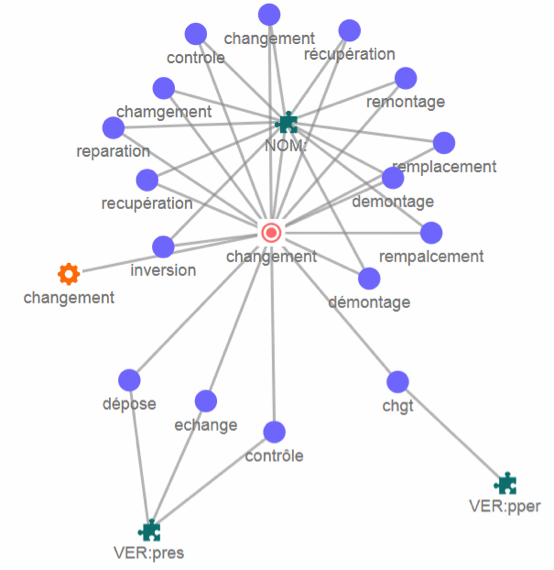
\includegraphics[width=6cm]{figures/w2v}
    \end{center}
    \caption{Graphe sur le mot changement}\label{fig:w2v}
\end{figure}


Afin de visualiser les résultats de Word2Vec formatés en RDF, nous avons créé une première ontologie modélisée sur Word2Vec. Elle est un premier palier en vue du peuplement d'ontologies métiers.


\section{Evaluation}
Nous avons réalisé une analyse qualitative en considérant les termes présents dans le lexique métier constitué manuellement. L'apport de Word2Vec a ainsi pu être démontré, certains termes ayant été omis par l'humain. Nous avons ainsi pu détecter automatiquement les types d’éléments suivants :

\begin{itemize}
\item des pluriels (ex : « moteur », « moteurs »)
\item 	des abréviations (ex : pour « transfo », « transformateur », qui n’était pas présent dans le lexique constitué manuellement)
\item 	des fautes/mots collés (« bloc » et « dublock »)
\item 	des hyponymes (pour « équipements » on retrouve « modem », « serveur » etc.)
\item 	des mots de la même famille (ex : « ventilateur » et « ventilation »)
\item 	des synonymes (ex : pour « remplacement » on retrouve avec W2V « changement », « échange » etc.
\item 	des phénomènes de multilinguisme : pour le terme « contrôle » : « controle » sans accent, termes anglais associés plus ou moins bien orthographiés « cheik » et « check ».
\item 	pour le terme « arrêt » on retrouve « stop »

\end{itemize}

Il nous reste à présent à effectuer une analyse quantitative poussée pour établir le taux de rappel et de précision en injectant ces lexiques à notre chaîne de traitement. Cette étape pourra être facilitée par notre outil d’exploration de termes et par CuriosiText.


\section{Peuplement semi-automatique d'ontologies métiers}

Problématique du bruit

Nous avons développé une application web, Curiositext, permettant à un utilisateur non expert de visualiser les résultats de Word2Vec et de peupler semi-automatiquement une ontologie métier. Celle-ci est indépendante de l'architecture de l'application ce qui permet d'utiliser CuriosiText pour des cas d'usage très divers, sans dépendre d'un domaine spécifique. Dans un premier temps, l'utilisateur est invité à charger un corpus texte local ou peut effectuer une requête à l'aide d'Elastic Search pour récupérer des données distantes. Il peut ensuite appliquer Word2Vec sur ses données. Les paramètres de base de la méthode sont paramétrables à savoir :

\begin{enumerate}
\item	la dimension des vecteurs,
\item	la taille de la fenêtre,
\item		la fréquence minimale d'apparition d’un terme pour l’apprentissage,
\item	le modèle (CBOW ou Skip-Gram),
\item	le nombre d’itérations.
\end{enumerate}

\begin{figure}[tb]
    \begin{center}
        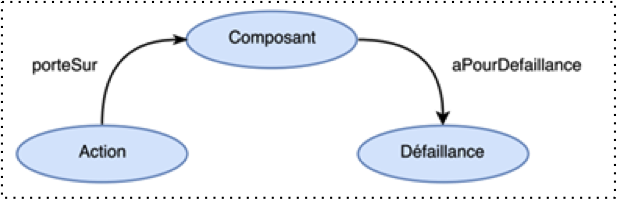
\includegraphics[width=6cm]{figures/ontMetier}
    \end{center}
    \caption{Ontologie métier}\label{fig:metier}
\end{figure}

L'utilisateur accède ensuite à la troisième partie de l'application à savoir le peuplement d'une ontologie. Il doit charger l’ontologie métier (fig \ref{metier}) développée en amont à peupler. Pour ce faire, nous avons mis en place un scénario de peuplement de l'ontologie finale illustré ici par la requête du terme "changement".
Pour aider au peuplement de l'ontologie, une ontologie linguistique (fig \ref{ling} a été intégrée dans l'application. L'utilisateur doit renseigner pour le terme requêté sa classe lexicale (Terme\_Canonique) et sa classe métier (Action).

\begin{figure}[tb]
    \begin{center}
        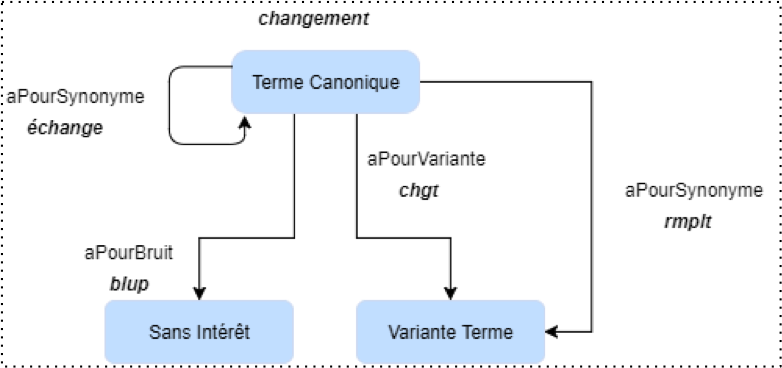
\includegraphics[width=8cm]{figures/ontLing}
    \end{center}
    \caption{Ontologie linguistique}\label{fig:ling}
\end{figure}



L'intérêt d'utiliser directement un entrepôt RDF comme backend de l'application nous permet de bénéficier, en plus des capacités de requêteage et de stockage, les possibilités de raisonnement définies lors de la création des ontologies. En effet, les déductions effectuées par l'entrepôt permmettent à l'interface de ne fournir que les informations minimales à celui-ci : il se charge de compléter celles-ci à l'aide de la formalisation OWL (RL)\cite{owlprofiles} définie dans les ontologies. Par exemple, le fait d'ajouter un lien de synonymie ou de variance dans les données va permmettre éventuellement de déduire l'appartenance d'un individu à une classe métier (ici Action) grâce à l'axiome ci-dessous\footnote{Notons que nous sommes obligé de dupliquer ce type d'axiome pour chaque classe concernée.
} :
$$
\begin{array}{ll}
\exists  \ \texttt{aPourSynonyme} .  \texttt {Action}  \sqcup \exists  \ \texttt{aPourVariante} .  \texttt {Action}
\sqsubseteq    \texttt{Action}
\end{array}
$$
En logique de description, cela signifie que tout individu qui a un synonyme ou une variante dans la classe Action appartient à la classe Action lui-même. Nous faisons la même chose pour les classes Composant et Defaillance, la logique du premier ordre ne nous permettant pas d'écrire des axiomes sur des ensembles de classes.
L'interface ne fait que qu'ajouter ou retirer des triplés RDF élémentaires, l'intelligence de l'entrepôt se charge de faire les mises à jour déclenchées par le raisonnement et éventuellement de détecter des incohérences dans les données.


\section{Conclusion et perspectives}
-	Évaluer quantitativement
-	Évaluer l'apprentissage Word2Vec avec et sans étiquetage morphosyntaxique pour montrer l'apport.
-	Utiliser l'ontologie peuplée semi-automatiquement comme corpus de référence pour de l'apprentissage supervisé en vue de la détection automatique de termes pertinent. Cela permettrait de réduire la tâche d'annotation de classes et de relations.
-	Tester le paramétrage de Word2Vec sur les expressions multi-mots.





\bibliographystyle{taln2018}
\bibliography{references}
%% commande no-cite pour inclure dans la bibliographie des références
%% qui ne sont pas citées dans le corps de l'article
\nocite{}

%%================================================================
\end{document}
